\documentclass[condensed]{union-cs-thesis}

% made a fresh document to write the draft

\usepackage{graphicx}
\usepackage[hidelinks]{hyperref}
\usepackage{cite}
\usepackage{fancyref}

% these packages are being used to allow for margin notes for editing
%\usepackage{marginnote}
%\usepackage[top=1.5cm, bottom=1.5cm, outer=5cm, inner=2cm,
 % heightrounded, marginparwidth=4cm, marginparsep=.5cm]{geometry}
% new command that makes leaving notes in the margin a little more friendly
%\newcommand{\editnote}[2]{\marginnote{\footnotesize #1}[#2]}
  

\graphicspath{ {./images/} }

%------------------------------------------------------------
\begin{document}

\title{Generative Models of Biological Ontogeny:\\\Large Evolving Skate Guts}
\author{Andrew Hilton}
\date{\today}

\maketitle
%------------------------------------------------------------
\begin{abstract}
\makeabstract
In Biology the idea that Ontogeny recapitulates Phylogeny allows Biologists to make inferences about the
Evolutionary history of an organism by examining the development of the organism from its embryonic
state through maturity.  While this allows for observations regarding the Evolutionary phases, it does
not give much indication of the environmental constraints and evolutionary pressures that caused
the changes.  Using Genetic Algorithms and Generative Encodings to model the development of skate intestines
we hope to confirm the well accepted evolutionary pressures that are believed to have caused their
unique shape.  This paper will discuss work that has already been done in relation to generative
encodings, as well as the proposed work for this project.

\end{abstract}

%------------------------------------------------------------
\section{Introduction}

\par
Within Biology there is a theory called Recapitulation theory that states ``Ontogeny recapitulates
Phylogeny.''  In essence this means that although most organisms begin their development in a similar
state, throughout the course of their Ontogeny (the development from embryo to mature organism) they
differentiate themselves from each other in a way that seemingly mirrors the evolution of their species.
Because of this, Biologists are particularly interested in examining the ontogeny of organisms, as a
means of approximating the phylogenetic changes that cause splits between species.

\par
One family of organisms whose ontogeny is of some interest are fish of the family \emph{Rajidae}, also
known as skates (see figure~\ref{fig:skatepic}).
\begin{figure}[h]
  \centering
  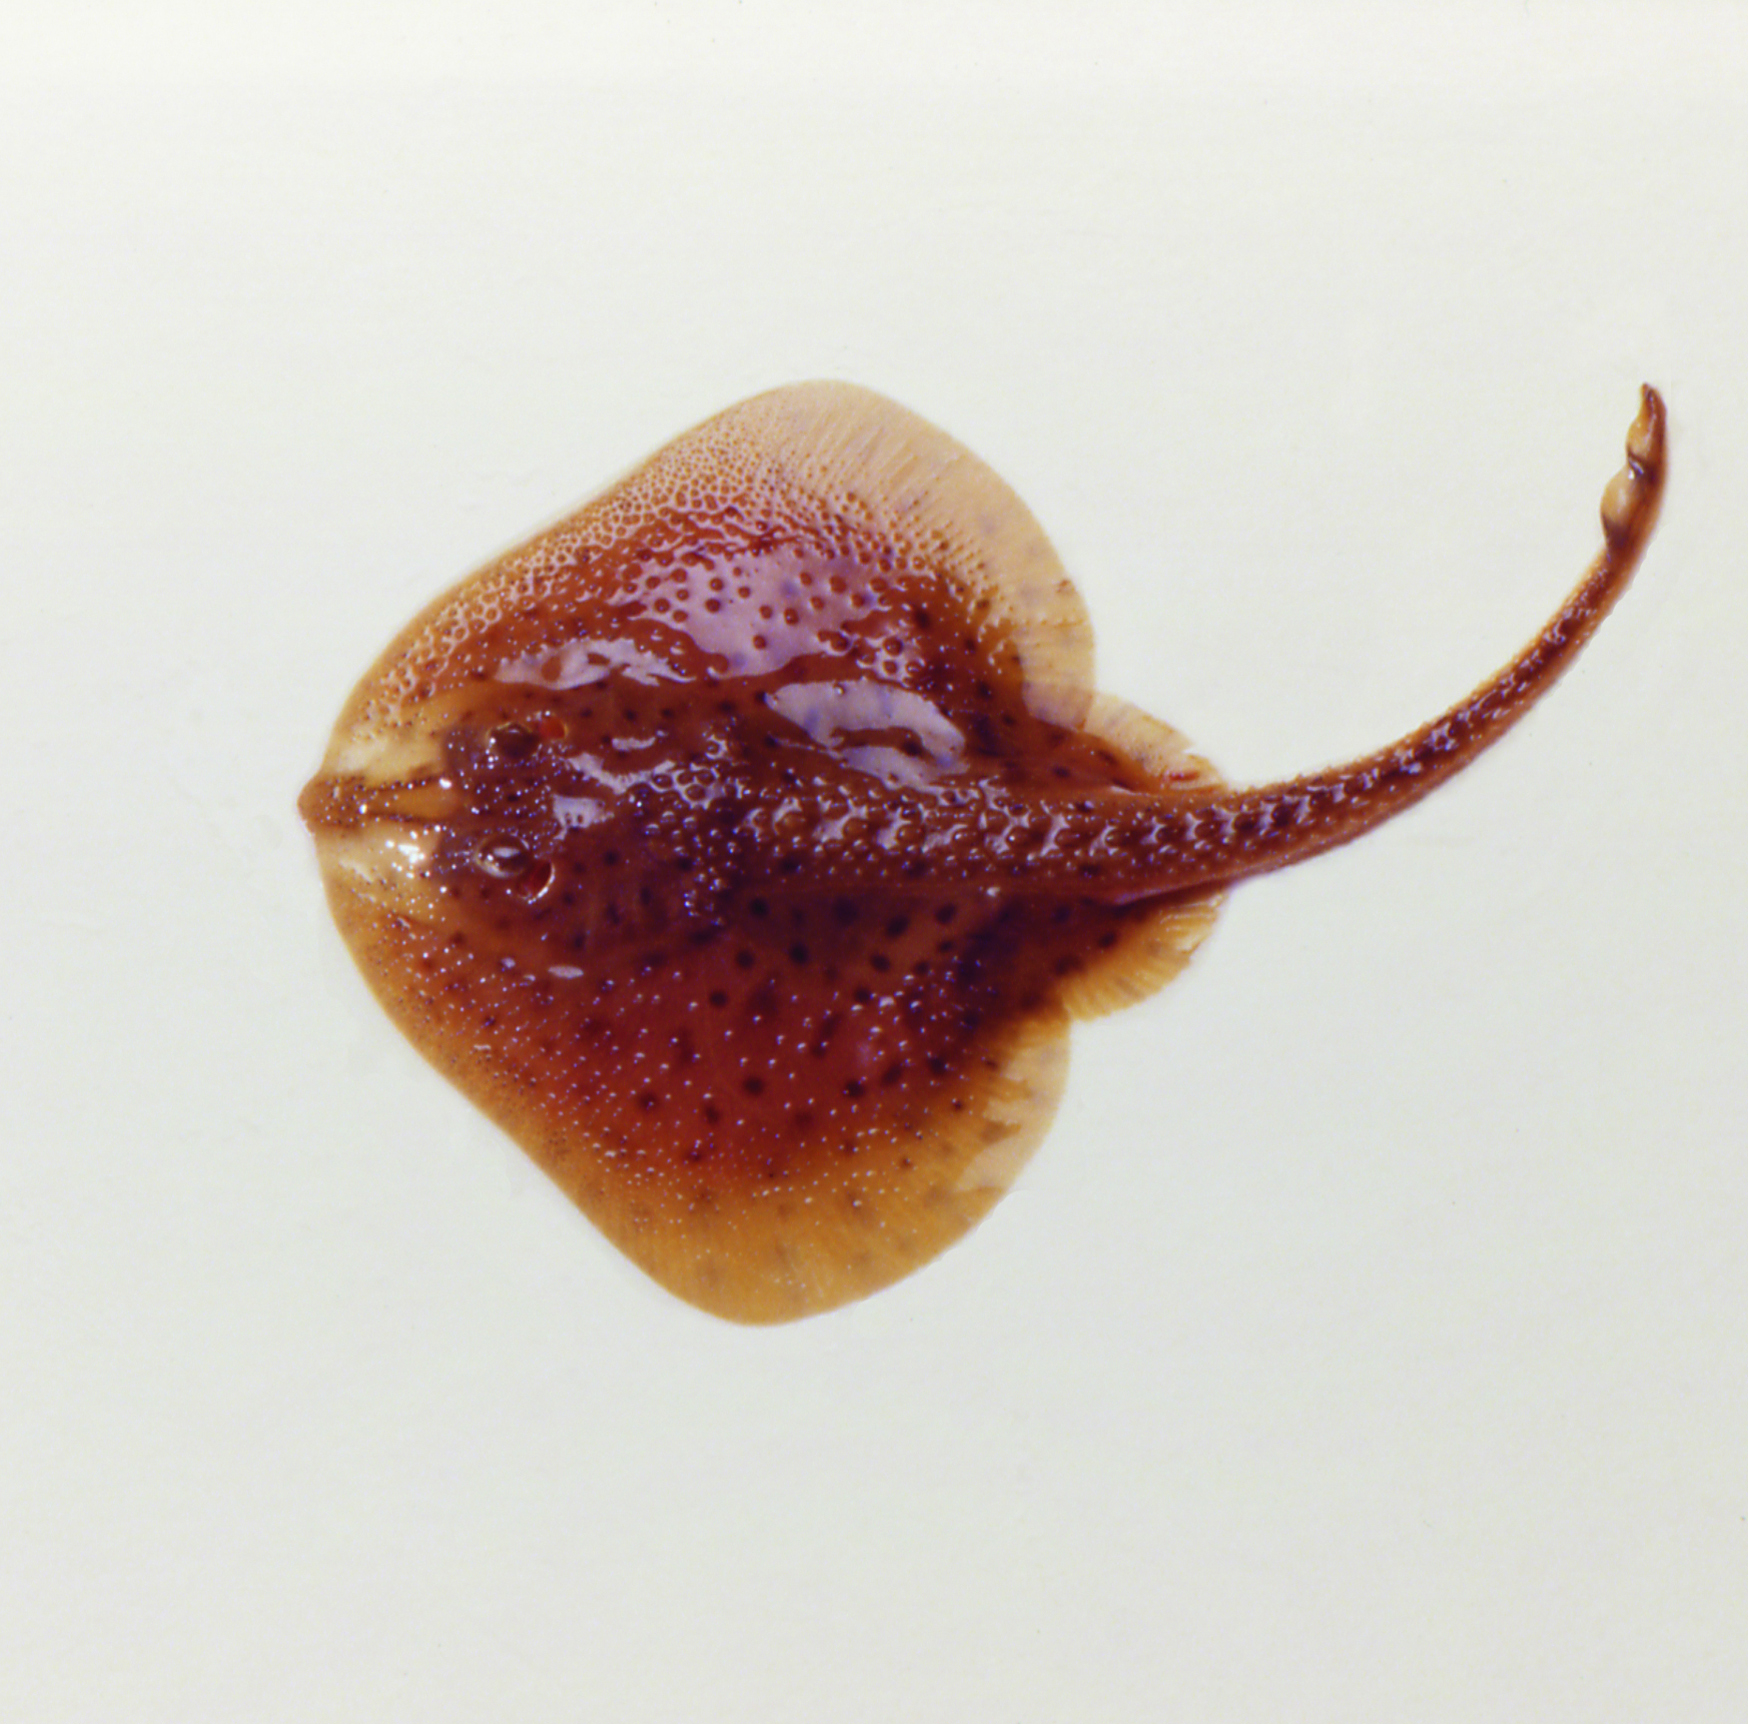
\includegraphics[scale=0.25]{skate-pic}
  \caption{A picture of a skate}
  \label{fig:skatepic}
\end{figure}
Skates are interesting from a biological standpoint largely due to their age (the predecessors to
the modern Rajidae family are thought to have developed nearly 450 million years ago), but also due to
the shape of their intestinal tract.  Like humans, skates consume a protein heavy diet, which due to the
nature of protein, requires much more digestive work to be done in order to absorb all of the necessary
nutrients.  In order to meet this requirement, humans and our predecessors developed long, winding
intestines that, when uncoiled, extend for more than twice our height.  Skates however are a type of
cartilaginous fish (skeletons are formed from cartilage rather than bone).  As such they do not have
the abdominal structure to support this shape of organ.  For this reason skate intestines have developed
as a contained volume, which has a twisting internal structure (see figure~\ref{fig:gut_model}).
\begin{figure}[h]
  \centering
  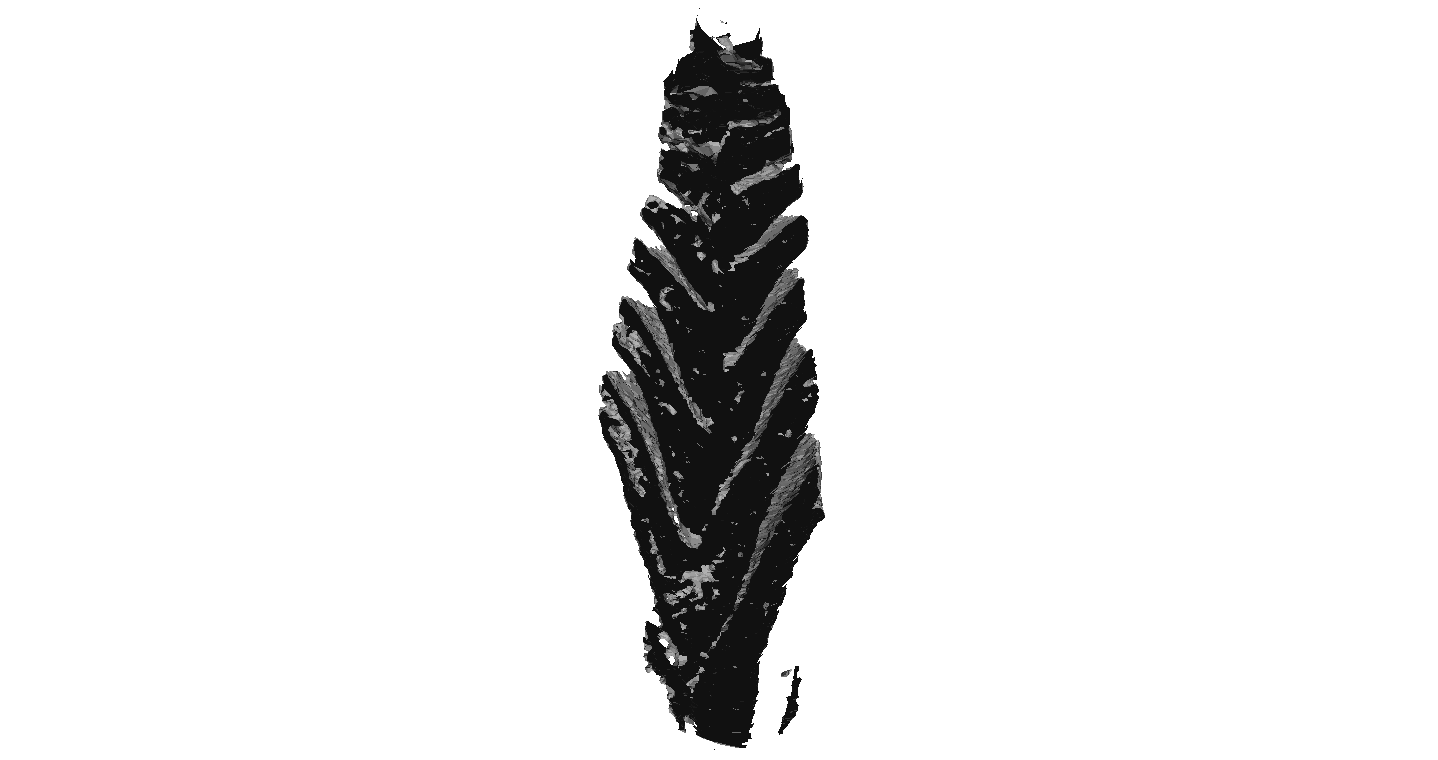
\includegraphics[scale=0.25]{model_img}
  \caption{A 3D model of the internal membrane of a skate intestine, created through CT-scans}
  \label{fig:gut_model}
\end{figure}

\par
While these reasoning behind these claims is biologically sound, and widely accepted, it is not known for
a fact that these are the constraints that led skates to evolve the way that they did.  However using
Recapitulation Theory it may be possible to test the accuracy of these claims.  A well-known method of
problem solving within Computer Science is the use of Genetic Algorithms.  In Genetic Algorithms potential
solutions are tested against a chosen fitness function, and then solutions are ``evolved'' and the process
is repeated.  Another related technique is that of \emph{Generative Encodings}.  A generative encoding is an
evolvable representation that allows the system to encode successful parts of a solution of a genetic algorithm
and use it as a building block in future solutions.  Using a generative encoding it may be possible to
evolve shapes that are similar tothose seen in skate intestines.  Using these techniques we will try to test
the actual effect that the above environmental constraints have on the shape of developing skate intestines.

%------------------------------------------------------------
\section{Related Works}
\label{sec:relatedworks}
\par
While the use of Genetic Algorithms is nothing new within the field of Computer Science, and their
applications are continually being investigated and expanded upon, this particular type of application
appears to be largely unexplored.  Even though GAs have long been used in various fields, and Biology
is far from being an exception, it does not appear as though much research has been done into
creating evolutionary representations of developing biological systems.  However much work has been
done in exploring the potential uses of Generative Encodings.  Various investigations in the field of
robotics have shown that Generative Encodings can be used to develop novel designs for soft-robots
\cite{rieffel2009automated},
as well as generating designs for antennae to be used in various satellite
\cite{lohn2005evolved}.
As was shown in Greg Hornby's work in developing a system for the creation of novel table designs, the
core concept behind Generative Encodings allows for the system to evolve encodings that are much more
complex, and as a general rule much more viable in terms of matching the physical constraints of the
objects themselves
\cite{hornby2004functional,hornby2001advantages}.

%% \par
%% Some of the work done by Josh Bongard deals with an interesting subset of evolutionary design,
%% namely the area of ``artificial ontogeny,'' i.e. using the concepts of generative encoding to find
%% solutions to various tasks by evolving artificial pseudo-organisms
%% \cite{bongard2002evolving}.
%% Despite it's surface-level relation to my topic area, most of Bongard's work has been in the field
%% of modular robotics, which uses small identical robotic ``cells'' to create functional multi-celled
%% robots that are capable of self-modifying in order to adapt to different situations.  While this is
%% not directly related to the proposed project, it is interesting to see that the idea of ontogeny is
%% already being used in the field of evolutionary representations.

\par
Despite this specific type of problem not being widely investigated, some of the work done by Marc
Toussaint has some overlap with the type of work planned for this project.
Toussaint's study has shown that evolving a grammar-based encoding of artificial plants produces more
effective solutions within fewer generations on average than a direct encoding
\cite{toussaint2003demonstrating}.\footnote{in this case the ``problem'' that solutions were trying to
  solve was how to maximize the plant's exposure to the sun}
The underlying thought behind the work done by Toussaint was the idea that a single phenotype
\footnote{the physical manifestation of genetic encoding}
could be represented by more than one genotype.
\footnote{a string of genetic information, a specific type of gene}
Toussaint was able to show that using a Genetic Encoding of an object allowed for multiple solutions
of similar shape be evolved, while having different underlying genetic represenations.  His work also
showed that using Generative Representations increased the overall effectiveness of the evolved
solutions, generating more fit solutions within fewer generations.  This lends itself to the strength
of Generative Encodings in regards to the proposed project, as the desired phenotype is already more
or less known, so the question lies more in what are the genotypes that lead to this trait.  Toussaint's
work also deals with grammar-based representations, which are of interest as we look to model the full
development of the skate intestine.  However the representations of plants he uses may be too simple
to be fully translatable to the more complex shapes of the skate organs.

%------------------------------------------------------------
\section{Planned Work}

%---------------------------------------------
\subsection{Approach}

In order to test the influence of environmental constraints on the development of skate intestine's
distinctive shape, we must see how shapes held to the same measures of fitness evolve and match how
closely related these evolved shapes are to those we can observe in actual skates.  As such we it makes 
sense to use a system that uses similar principles to real evolution, namely measures of fitness and
propagation of and alteration of successful solutions through generations.  It is for this reason that
an approach implementing genetic algorithms is being proposed for this project.  Genetic algorithms are
built on the ideas that by combining parts of successful solutions will eventually lead to solutions that
are even more fit to solve the local problem \cite{mitchell1998introduction}.  By mimicking the concepts
of reproduction and mutation, genetic algorithms have been used to solve many complex problems across
various fields.  While it would be incorrect to say that genetic algorithms in the context of this problem
would allow us to model the actual evolution of skate intestines, they do provide a tool that is capable
of showing how shapes would develop under different constraints, which is the goal of the research question.

\par
Much of the work that has been done in regards to using genetic algorithms to evolve shapes have discovered 
that employing a method known as generative encodings (also known as generative representations) produces
much more effective results (as discussed in section ~\ref{sec:relatedworks}).  In order to produce shapes
that more closely resemble actual physical organs, we plan on employing a generative encoding.  However
there are many different strategies in creating generative representations, and at this point it is difficult
to decide which of the methods that have been discussed would best fit the research we hope to do.  As such,
the early work that will be done for this project will be in continuing to investigate the various approaches
of creating generative encodings in order to decide which technique best fits the requirements of this project.

\par
While the techniques discussed in the related works section are not a conclusive list, they represent a starting
point of the research that will be continued in the next part of the project.  The approaches that have been seen
so far can be broken down into 3 basic categories.

\begin{description}
\item[Graph Based Encodings]\cite{rieffel2009automated} \\ 
This type of encoding was used in the work done by Rieffel
et al, in their work on developing irregular designs for tensegrities.  In this approach 3D structures are
represented by graphs, where nodes are numbered in pairs which represent the struts of the tensegrity shape, and the
edges between nodes are used to represent the tensile elements of the structure.  This type of representation does
not fit the type of shape we hope to create as the structures generated by this type of representation do are very
simple and geometric in shape.  Due to the nature of tensegrities as simple structures composed of just struts and
tensile elements, this type of representation is very well suited, however it does not have much application outside
of this.
\item[Grammar Encodings]\cite{toussaint2003demonstrating,hornby2004functional} \\
The use of grammar based encodings to generate shapes seen in nature is not a particularly new idea 
\cite{prusinkiewicz2012algorithmic},
however using a grammar based generative encoding has shown to be very effective in generating various different types
of shapes.  In the work done by both Toussaint and Hornby, a grammatical l-system was used to produce the shapes in
the studies.  
\par
Hornby's study was in creating novel designs for tables based on an initial configuration.  The representation used
was encoded as a series of instructions for a turtle, which would then move around a 3D space filling in space as it
traveled.  While they were able to generate complex structures, due to the nature of their goal and the system they used
the shapes produced were too geometrically regular in nature, being constrained to orthogonal directions.  The models that
we are trying to generate are based on biological models and are therefore much more irregular and require smoother models
\par
The goal of Toussaint's study was in generating artificial plants, and did not need very detailed models
of the shapes themselves.  Therefore the grammars used in his study produced simple branch like structures.  While the
hope for this project is that we will be able to produce more complex 3D shapes, a system similar to the one used by
Toussaint may be useful as a starting point to create simpler models, and later on, more overhead may be able to be
introduced into the system to create the more complete shapes that we are aiming for.
\item[CPPNs] \cite{clune2010investigating} \\
\emph{Compositional Pattern Producing Networks} also known as CPPNs are a type of representation used in the work done on the
HyperNEAT network \cite{clune2010investigating}.  These types of networks use a combination of both sinusoidal and 
sigmoid functions to produce images that can seem natural and irregular.  Some work has been done in combining these networks
with both Neural Networks and genetic algorithms, and given the nature of the shapes that we will be working with for
this project, CPPNs show some promise and will require further investigation.
\end{description}

\par
Once an appropriate type of network has been representation has been selected, the main part of the investigation
will begin.  The main approach that will be used in this project will be in doing runs of genetic algorithms over
the representations and examining the results.  To start, various fitness functions will be selected to explore
how the constraints given would alter the shape of the resulting shapes.  The selection of these parameters will
require further collaboration with faculty within the Biology Department in order to determine what kind of 
constraints seem reasonable to test.  Based on conversations that have already been had with Professor Theodosiou
(the main researcher at Union working with skates and their development) one of the early measures of fitness
that will be used is by exploring how constraining the shape to a fixed enclosing volume, and trying to maximize
the internal surface area (to simulate the exposure of digested food the absorbing surface) affects the resulting shape.
As more trials are run, the fitness functions will be altered by adding more complexity to them, and the initial
configurations will be changed to explore if the starting point of the shape has an effect on the outcome.

%---------------------------------------------
\subsection{Evaluation}

Given the time constraints of this project, it will be difficult to perform a full quantitative analysis
of the results (in terms of accuracy of models to shape of real skate intestines).  Fortunately it won't be
necessary to justify the results with absolute mathematical precision when a qualitative analysis will
yield a strong enough result.  The baseline for the evaluation of success will be whether or not the models
begin to develop shapes that have the signature twisting structure, and how much they resemble skate guts in
a basic comparison.
\par
However enough headway is made early on in the project and the models begin to look promising early on, there
are techniques using differential geometry that could be used to compare the models generated by the genetic
algorithm, and models based on real skate intestines.
%In this case an analysis would be done on using the models generated by Union College's own Professor Theodosiou and her students
%\par
%While the main goal of this project is to see if these constraints lead to shapes that resemble the shapes seen
%in skates, this is not the only interesting result that may be seen.  There is potential that through 

%------------------------------------------------------------
\section{Timeline}

\begin{description}
\item[Fall] Much of the work that will be completed in the early part of the Fall term will be towards continuing
  research into the topic.  A large portion of this research will be focused on looking into potential techniques
  and systems for creating and evolving generative representations.  This will involve continuing reading
  about the different systems, but also investigating hands on which systems produce the best results for
  the project, and are easiest to use.
  \par
  Once a suitable system has been decided on, preliminary testing of the generative encodings will begin.
  These tests will start with simple fitness functions and initial configurations.  As more tests are run
  the parameters of the test will be altered to see if there are potentially other factors that must be
  consideredl, or if there must be certain initial conditions to get satisfactory results.
\item[Winter] The Winter term will be largely focused on continuing to run trials, and beginning to synthesize the
  results of the tests.  If sufficient progress had been made during the Fall term, then some of the work
  done in the late Fall and Winter could be towards finding and using a method of geometric analysis, in order
  to quantitatively describe the success of the project.
\end{description}


\bibliographystyle{plain}
\bibliography{centralbib}

\end{document}
